% This is text associated with the open textbook "Open Electromagnetics"
% See immediately below for author, date
% This work is licensed under the Creative Commons Attribution-ShareAlike 4.0 International License. (CC BY-SA 4.0) 
% To view a copy of the license, visit http://creativecommons.org/licenses/by-sa/4.0/

%ORB TITLE Friis Transmission Equation
%ORB AUTHOR 0        # S.W. Ellingson, Virginia Tech (ellingson@vt.edu)
%ORB DATE 20191212   # yyyymmdd
%ORB ABSTRACT 

\label{m0219_Friis_Transmission_Equation} % <-- Must match name of this file and module directory name.  Don't mess with this!
\index{Friis transmission equation|(}

A common task in radio systems applications is to determine the power delivered to a receiver due to a distant transmitter.
The scenario is shown in Figure~\ref{m0219_fFTE}:
%
\begin{figure}[b!] % <--- "[b!]" for first figure in section *only*; delete for 2nd and subsequent figures
\begin{center}
\pdftooltip{{  % note double braces
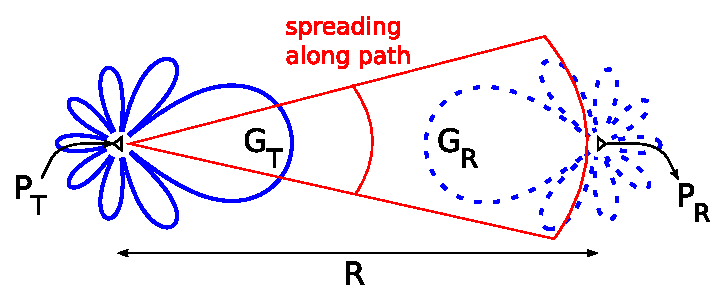
\includegraphics[width=\columnwidth]{modules/m0219_fFTE.eps} 
% https://en.wikipedia.org/wiki/File:Sidelobes_en.svg
}}{Two half-power beamwidth patterns side-by-side. The right side pattern is the mirror image of the left and drawn with a dashed line. The left pattern is capital P subscript capital T and main lobe capital G subscript capital T. A triangular arc spreads from the left pattern and encompasses the main lobe of the second pattern. The second pattern has main lobe capital G subscript capital R and is capital P subscript capital R. The patterns are a distance capital R from center to center. 
}
\end{center}
%\centerline{\scriptsize 
%\copyright~\hyperref[m0205_Sidelobes_Credit]{T.\ Truckle} 
%\href{https://creativecommons.org/licenses/by-sa/4.0/}{CC BY-SA 4.0} 
%(modified) 
%} % \centerline 
\caption{
\label{m0219_fFTE}
Radio link accounting for antenna gains and spreading of the transmitted wave.
}
\end{figure}
%
A transmitter delivers power $P_T$ to an antenna which has gain $G_T$ in the direction of the receiver.
The receiver's antenna has gain $G_R$.
As always, antenna gain is equal to directivity times radiation efficiency, so $G_T$ and $G_R$ account for losses internal to the antenna, but not losses due to impedance mismatch.

A simple expression for $P_R$ can be derived as follows.
First, let us assume ``free space conditions''; that is, let us assume that the intervening terrain exhibits negligible absorption, reflection, or other scattering of the transmitted signal.
In this case, the spatial power density at range $R$ from the transmitter which radiates this power through a \emph{lossless and isotropic} antenna
\index{antenna!isotropic}
would be:
%
\begin{equation}
\frac{P_T}{4\pi R^2} 
\end{equation}
%
that is, total transmitted power divided by the area of a sphere of radius $R$ through which all the power must flow.
The \emph{actual} power density $S^i$ is this amount times the gain of the transmit antenna, i.e.:
%
\begin{equation}
S^i = \frac{P_T}{4\pi R^2} G_T
\end{equation}
%  
The maximum received power is the incident co-polarized power density times the effective aperture $A_e$ of the receive antenna:
%
\begin{flalign}
P_{R,max} &= A_e S^i_{co} \nonumber \\
          &= A_e \frac{P_T}{4\pi R^2} G_T \label{m0219_ePRmax1}
\end{flalign}
%
This assumes that the receive antenna is co-polarized with the incident electric field, and that the receiver is conjugate-matched to the antenna.
The effective aperture can also be expressed in terms of the gain $G_R$ of the receive antenna:
%
\begin{equation}
A_e = \frac{\lambda^2}{4\pi} G_R
\end{equation}
%
Thus, Equation~\ref{m0219_ePRmax1} may be written in the following form:
%
\begin{equation}
\boxed{
P_{R,max} = P_T G_T \left(\frac{\lambda}{4\pi R}\right)^2 G_R
\label{m0219_eFTE}
}
\end{equation}
%
This is the \emph{Friis transmission equation}.
Summarizing:
%
%%%%%%%%%%%%%%%%%%%%%%%%%%%%%%%%%%%%%%%%%%%%%%%
%ORB HIGHLIGHT
\begin{mdframed}[backgroundcolor=yellow!20,nobreak=true] 
The \emph{Friis transmission equation} (Equation~\ref{m0219_eFTE}) gives the power delivered to a conjugate-matched receiver in response to a distant transmitter, assuming co-polarized antennas and free space conditions.
\end{mdframed}
%%%%%%%%%%%%%%%%%%%%%%%%%%%%%%%%%%%%%%%%%%%%%%%

The factor $\left(\lambda/4\pi R\right)^2$
%%
%\begin{equation}
%\left(\frac{\lambda}{4\pi R}\right)^2 
%\end{equation}
%
appearing in the Friis transmission equation is referred to as \emph{free space path gain}.
\index{path gain}
More often this is expressed as the reciprocal quantity:
%
\begin{equation}
\boxed{
L_p \triangleq \left(\frac{\lambda}{4\pi R}\right)^{-2} 
}
\end{equation}
%
which is known as \emph{free space path loss}.
\index{path loss}
Thus, Equation~\ref{m0219_eFTE} may be expressed as follows:
%
\begin{equation}
P_{R,max} = P_T G_T L_p^{-1} G_R
\label{m0219_eFTE2}
\end{equation}
%
The utility of the concept of path loss is that it may also be determined for conditions which are different from free space.
The Friis transmission equation still applies; one simply uses the appropriate (and probably significantly different) value of $L_p$.

A common misconception is that path loss is equal to the reduction in power density due to spreading along the path between antennas, and therefore this ``spreading loss'' increases with frequency.
In fact, the reduction in power density due to spreading between any two distances $R_1 < R_2$ is:
%
\begin{equation}
\frac{P_T/4\pi R_1^2}{P_T/4\pi R_2^2} = \left(\frac{R_1}{R_2}\right)^2
\end{equation}
%
which is clearly independent of frequency.
The path loss $L_p$, in contrast, depends only on the total distance $R$ and does depend on frequency.
The dependence on frequency reflects the dependence of the effective aperture on wavelength.
Thus, path loss is not loss in the traditional sense, but rather accounts for a combination of spreading and the $\lambda^2$ dependence of effective aperture that is common to all receiving antennas. 

Finally, note that Equation~\ref{m0219_eFTE2} is merely the simplest form of the Friis transmission equation.
Commonly encountered alternative forms include forms in which $G_T$ and/or $G_R$ are instead represented by the associated effective apertures, and forms in which the effects of antenna impedance mismatch and/or cross-polarization are taken into account.

%%%%%%%%%%%%%%%%%%%%%%%%%%%%%%%%%%%%%%%%%%%%%%%
%ORB EXAMPLE
~\\ \begin{example} 
\begin{mdframed}[backgroundcolor=brown!20,linecolor=brown!20]\raggedright
6~GHz point-to-point link.
\\~\\
Terrestrial telecommunications systems commonly aggregate large numbers of individual communications links into a single high-bandwidth link.
This is often implemented as a radio link between dish-type antennas having gain of about $27$~dBi (that's dB relative to a lossless isotropic antenna) mounted on very tall towers and operating at frequencies around 6 GHz.
Assuming the minimum acceptable receive power is $-120$~dBm (that's $-120$~dB relative to 1~mW; i.e., $10^{-15}$~W) and the required range is 30~km, what is the minimum acceptable transmit power?\\
%
~\\
{\bf Solution.} From the problem statement:
%
\begin{equation}
G_T=G_R=10^{27/10}\cong 501 
\end{equation}
%
\begin{equation}
\lambda =\frac{c}{f} \cong \frac{3 \times 10^8~\mbox{m/s}}{6 \times 10^9~\mbox{Hz}} \cong 5.00~\mbox{cm} 
\end{equation}
%
$R=30$~km, and
$P_R\ge 10^{-15}$~W.
We assume that the height and high directivity of the antennas yield conditions sufficiently close to free space.
We further assume conjugate-matching at the receiver, and that the antennas are co-polarized.
Under these conditions, $P_R=P_{R,max}$ and Equation~\ref{m0219_eFTE} applies.
We find:
%
\begin{flalign}
P_T &\ge \frac{ P_{R,max} }{ G_T \left(\lambda/4\pi R\right)^2 G_R } \\
    &\cong 2.26 \times 10^{-7}~\mbox{W} \nonumber \\
    &\cong 2.26 \times 10^{-4}~\mbox{mW} \nonumber \\
    &\cong \underline{-36.5~\mbox{dBm}} \nonumber
\end{flalign}

\end{mdframed}
% note figures will need to go between "\end{mdframed}" and "\end{example}"
\end{example}
%%%%%%%%%%%%%%%%%%%%%%%%%%%%%%%%%%%%%%%%%%%%%%%


%%%%%%%%%%%%%%%%%%%%%

{\bf Additional Reading:}
\begin{itemize}
\item ``\href{https://en.wikipedia.org/wiki/Free-space_path_loss}{Free-space path loss}'' on Wikipedia.
\item ``\href{https://en.wikipedia.org/wiki/Friis_transmission_equation}{Friis transmission equation}'' on Wikipedia.
\end{itemize}

%%%%%%%%%%%%%%%%%%%%%%

\index{Friis transmission equation|)}

